\chapter{Tinjauan Pustaka}

\par
Dalam suatu analisis diperlukan dukungan hasil-hasil analisis yang telah ada sebelumnya yang berkiatan dengan penetian tersebut.

Menurut Dwi Prastowo Darminto {(2002;52)} Analisi adalah Penguraian suatu pokok atas berbagai bagiannya dan menelaah bagian itu sendiri serta hubungan antar bagian untuk memperoleh pengertian yang tepat dan pemahaman arti keseluruhan.

Menurut Komaruddin {(2001:53)} Pengertian analisis adalah kegiatan berpikir untuk menguraikan suatu keseluruhan menjadi komponen sehinga dapat mengenal tanda-tanda komponen, hubungannya satu sama lain dan fungsi masing-masing dalam satu keseluruhan yang terpadu.

Dengan demikian, bisa disimpulkan bahwa pengertian analisis yaitu suatu prosedur tahapan pekerjaan yang akan didokumentasikan dengan tahapan pembuatan laporan agar mudah dalam pemahaman.

\section{Selenium}
Selenium adalah perangkat lunak yang berfungsi untuk mendukung
pengembangan otomatisasi uji berbasis web aplikasi. Selenium menyediakan pengujian khusus terhadap domain bahasa,untuk melakukan tes menulis pada beberapa bahasa pemrograman yan populer, termasuk C\#, Groovy, Java, Pearl,PHP, Python, Ruby, dan juga Scala \cite{razak2011agile}. Pengujian dapat berjalan melalui browser web apa saja dan dapat dilakukan melalui Sistem Operasi di Windows, Linux, dan Platform OS X. Selenium Python Bindings menyediakan API yang sederhana untuk menulis uji fungsional menggunakan Selenium WebDriver, dan juga dapat mengakses semua fungsi Selenium WebDriver secara intuitif. Selenium Python Bindings menyediakan API yang cukup nyaman untu melakukan suatu akses Selenium WebDrivers seperti di Firefox, Internet Explorer, Chrome, dll
Ada beberapa alat Selenium untuk otomasi perangkat lunak diantaranya,Selenium IDE, Selenium RC, dan Selenium WebDriver.

\subsection{Selenium IDE}
Selenium IDE adalah lingkungan pengembangan yang terintegrasi untuk membangun suatu skrip yang akan diujikan. Ini adalah suatu plug-in Firefox yang memungkinkan merekam edit dan juga men-debug suatu kasus uji di selenium\cite{razak2011agile}. Ini mencatat semua tindakan yang dilakukan oleh pengguna yang skrip pengujian. Fitur yang terdapat pada Selenium IDE yaitu: Kemudahan untuk recorcd dan playback, Seleksi field yang pintar menggunakan id, nama, class, XPath dan lainnya sesuai kebutuhan, Auto complete untuk semua perintah selenium yang umum, wakl through test (step by step), debug dan pengaturan breakpoint, menyimpan script test sebagai HTML, Phyton, Ruby, dan format lain, Mensupport file Selenium user-extensions.js, OPsi untuk secara otomatis mengecek judul setiap halaman, kemudahan melalui plugins.

\subsection{Remote Control Selenium}{(RC)}
Remote Control Selenium (RC) adalah selenium utama yang digunakan untuk memproyeksikan waktu yang lama. Selenium RC lebih lambat daripada selenium webdriver karena menggunakan program java script yang disebut sebagai suatu inti dari selenium \cite{maruyama1994wireless}. Selenium RC harus memulai server sebelum menjalankan suatu skrip pengujian, dan itu tidak mendukung untuk aplikasi Ajax. Cara menghindari keterbatasan Selenium RC, yaitu dengan selenium WebDriver. Selenium RC terdiri dari dua bagian yaitu:
\begin{enumerate}
    \item Server yang secara otomatis menjalankan dan menghentikan web browser, dan bertindak sebagai HTTP proxy untuk setiap web request. Server menggunakan java.
    \item Librari Client untuk Bahasa pemograman Java, Python, PHP, Perl, Ruby, dan C\#.
\end{enumerate}

\subsection{Selenium WebDriver}
Secara langsung berkomunikasi dengan browser, jadi selenium WebDriver menyebabkan lebih cepat daripada Selenium RC. Selenium WebDriver mendukung beberapa browser web dan juga mendukung untuk aplikasi Ajax \cite{razak2011agile}. Tujuan utama dari Selenium WebDriver untuk meningkatkan dukungan modern masalah pengujian aplikasi di berbagai web, dan juga mendukung berbagai bahasa untuk menulis suatu skrip pengujian. Terlepas dari semua keunggulan Selenium WebDriver, ia memiliki keterbatasan pada saat menguji suatu aplikasi web, karena tidak memiliki fungsionalitas untuk menghasilkan tangkapan layar dalam kasus uji kegagalan. Selenium WebDriver tidak memiliki kapabilitas bawwan untuk menghasilkan hasil dari tes, dikarenakan tergantung pada pihak alat ketiga untuk menghasilkan laporan pengujian. Keterbatasan ini dapat dihindari dengan menggunakan kerangka TestNG

\subsection{TestNG}
TestNG adalah kerangka kerja pengujian yang dirancang untuk mengatasi keterbatasan kerja dari pengujian Jumlah unit. TestNG mencakup semua kategori tes sebagai unit, fungsional, pengujian integrasi. TestNG menghasilkan laporan pengujian dan menjalankan beberapa tes case secara paralel. Laporan TestNG sangat membosankan untuk diahami, sehingga memerlukan beberapa modifikasi.

\subsection{Selenium Grid}
Server yang memungkinkan pengujian untuk menggunakan instace browser web yang sedang berjalan di mesin jarak jauh. Dengan selenium grid, satu server bertindak sebagai hub\cite{razak2011agile}. Tes hubungi hub untuk mendapatkan akses ke instance browser karena hub memiliki daftar server yang menyediakan akses ke insntance browser (node WebDriver), dan memungkinkan pengujian menggunakan instance ini. Selenium Grid memiliki kemampuan untuk menjalankan tes pada instance browser jarak jauh yang berguna untuk menyebarkan beban pengujian di beberapa mesin, dan untuk menjalankan tes di browser yang berjalan pada platform atau sistem operasi yang berbeda. Yang terakhir ini sangat berguna dalam kasus di mana tidak semua browser yang akan digunakan untuk pengujian dapat berjalan pada platform yang sama.

\subsection{Selenium Core}
Bagian yang melakukan playback pada web browser yang sebenarnya.

\subsection{Analisis Sistem}
Analisis sistem adalah penelitian terhadap sebuah sistem dengan tujuan mengevaluasi berbagai macam masalah maupun hambatan yang muncul pada sistem aplikasi yang nantinya dapat dilakukan perbaikan atau pengembangan \cite{aini2007sistem}. Analisis penting dalam segala aspek dan sangat dibutuhkan untuk melakukan sebuah penelitian maupun pengembangan. Kemampuan dalam menganalisa suatu sistem juga diperlukan saat mempelajari bagaimana proses terciptanya aplikasi dan cara kerja sebuah aplikasi.

\section{Cara Install Selenium}
\begin{enumerate}
    \item Buka cmd, kemudian ketik python dan kemudian enter
    \item Langkah selanjutnya, ketik pip install selenium.
    \item Selanjutnya ketik list, untuk mengecek apakah selenium sudah terinstall di laptop anda

\end{enumerate}

\section{Anaconda}
Anaconda adalah perusahaan pengembang dan juga pengembang perangkat lunak pendukung sumber terbukayang berbasis di Austin, Texas, AS. Berkomitmen untuk open source, dan juga menciptakan distribusi dari Anaconda Python dan berkontribusi pada banyak alat analisis data berbasis sumber terbuka lainnya.

\subsection{Cara Install Anaconda}
Sebelum menginstall Anaconda Python hal pertama yang harus diperhatikan yaitu versi dari Sistem Operasi yang digunakan, misalnya Windows versi 32bit atau 64bit, jadi anda harus menginstall Anaconda Pyton sesuai dengan Sistem Operasi di windows anda, karena jika versi windows dapat menyebabkan error.
\begin{enumerate}
    \item Download Anaconda Python https://www.anaconda.com/distribution/
    \item Jika sudah didownload, buka installer Anaconda
    \begin{figure}[!htbp]
        \centering
        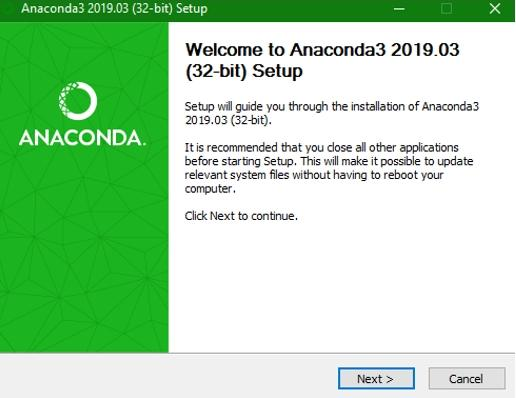
\includegraphics[scale=0.6]{figure/Anaconda/1.jpeg}
        \label{gambar 1}
    \end{figure}
    \vspace{2cm}
    \item Kemudian Pilih lokasi menyimpanan aplikasi
    \begin{figure}[!htbp]
        \centering
        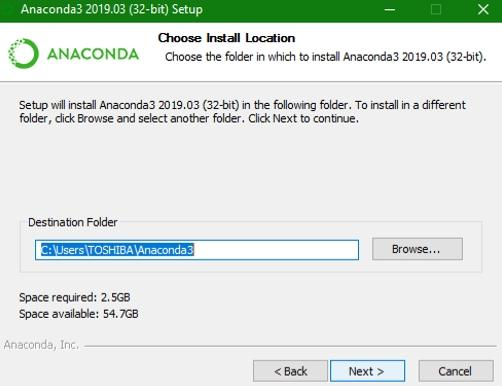
\includegraphics[scale=0.6]{figure/Anaconda/3.jpeg}
        \label{gambar 1}
    \end{figure}
    \item Lalu pilih Just Me(recommended) agar sesuai dengan computer yang ada miliki.
    \begin{figure}[!htbp]
        \centering
        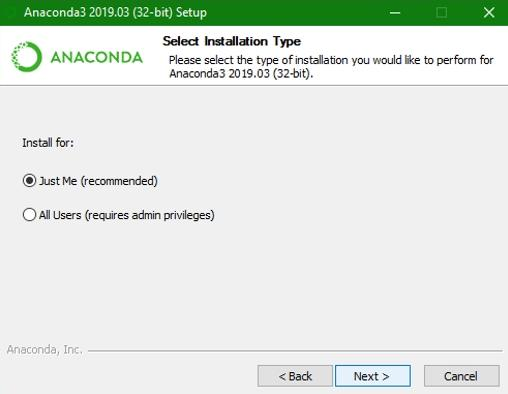
\includegraphics[scale=0.6]{figure/Anaconda/4.jpeg}
        \label{gambar 1}
    \end{figure}
           \vspace{2cm}
    \item Kemudian ceklis Add Anaconda to my PATH
    \item Lalu anda centang Add Anaconda to my Path environment variable, agar saat mengisntall selenium langsung ke path anaconda tidak ke aplikasi yang lain.
    \item Jika sudah klik install, tunggu sampai selesai proses installasi selesai.
    \begin{figure}[!htbp]
        \centering
        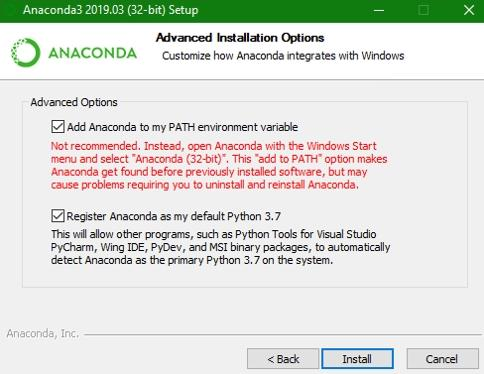
\includegraphics[scale=0.6]{figure/Anaconda/5.jpeg}
        \label{gambar 1}
    \end{figure}
    \item Klik Next  
    \begin{figure}[!htbp]
        \centering
        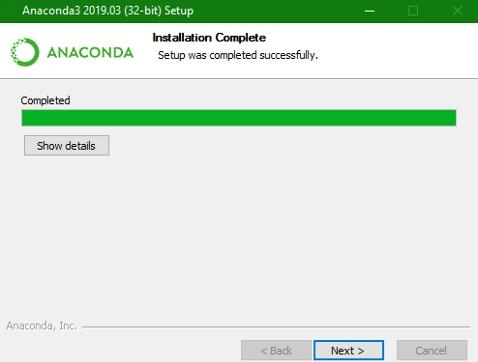
\includegraphics[scale=0.6]{figure/Anaconda/6.jpeg}
        \label{gambar 1}
    \end{figure}
    \vspace{2cm}
    \item Klik Next
    \begin{figure}[!htbp]
        \centering
        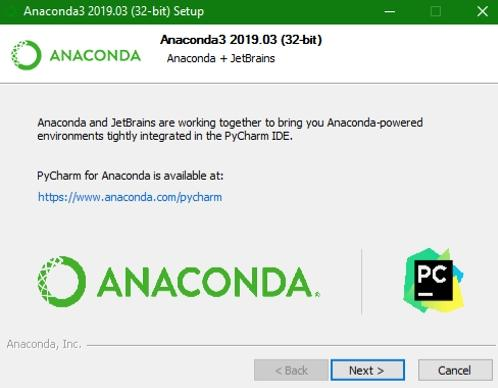
\includegraphics[scale=0.6]{figure/Anaconda/7.jpeg}
        \label{gambar 1}
    \end{figure}
    \item klik Next
    \item Jika sudah selesai Klik Finish
    \begin{figure}[!htbp]
        \centering
        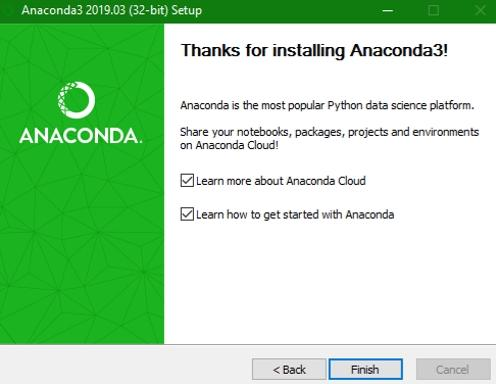
\includegraphics[scale=0.6]{figure/Anaconda/8.jpeg}
        \label{gambar 1}
    \end{figure}
\end{enumerate}
    \vspace{1cm}
\subsubsection{Flowchart}
Pengertian flowchart adalah bagan alir yang menggambarkan prosedur pada suatu sistem dengan simbul-simbol yang memiliki maknanya masing-masing \cite{solikin2018implementasi}. Fungsi dari flowchart yaitu untuk merancang proyek baru, menggambarkan proses bisnis, menggambarkan alur kerja dan menampilkan sebuah algoritma. Berberapa simbol yang ada pada flowchart yakni simbol arus, simbol proses dan simbol input/output. Pada gambar \ref{gambar 1} berikut contoh simbol simbol Flowchart.

\begin{figure}[!htbp]
    \centering
    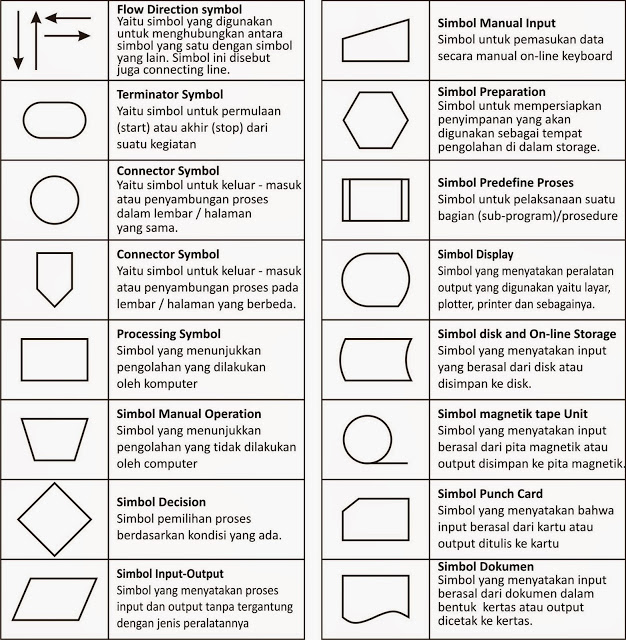
\includegraphics[scale=0.6]{figure/flowchart.jpg}
    \caption{\textit{Simbol Flowchart}}
    \label{gambar 1}
\end{figure}
\vspace{1cm}
\subsubsection{Flowmap}
Flowmap adalah penggambaran secara grafik sebuah prosedur yang ada pada suatu program \cite{rahayu2011perancangan}. Flowmap membantu analisis karena flowmap menggambarkan alur prosedur dan juga algoritma secara grafik. Pada gambar \ref{gambar 2} berikut contoh simbol simbol flowmap.

\begin{figure}[!htbp]
    \centering
    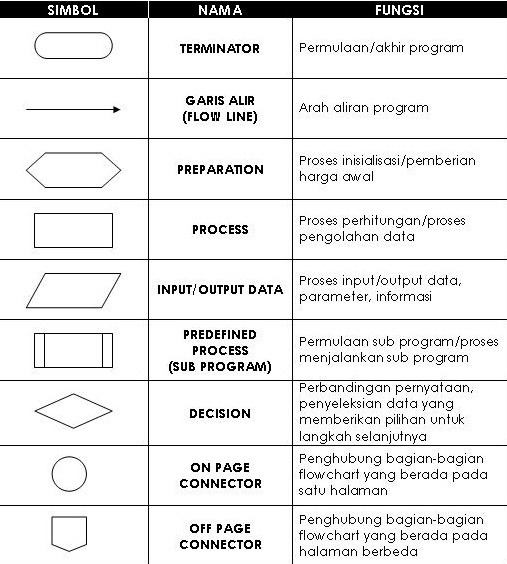
\includegraphics[scale=0.8]{figure/flowmapp.JPG}
    \caption{\textit{Simbol Flowmap}}
    \label{gambar 2}
\end{figure}
\vspace{4cm}
\subsection{Perancangan Sistem}
\subsubsection{Data Flow Diagram (DFD)}
Data Flow Diagram (DFD) adalah bentuk model hasil analisis sebuah kebutuhan dari perangkat lunak \cite{rivai2013pembangunan}. DFD bisa dikatakan sebagai gambaran rancangan sistem dari sebuah program yang berorientasi ke alur data dengan tujuan agar gambaran tersebut mudah dikomunikasikan oleh pembuat sistem atau pembuat program ke pengguna program tersebut.Pada gambar \ref{gambar 3} berikut contoh simbol simbol Dfd.

\begin{figure}[!htbp]
    \centering
    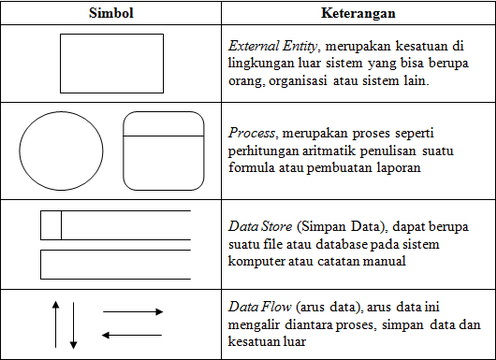
\includegraphics[scale=0.9]{figure/dfd.jpg}
    \caption{\textit{Simbol DFD}}
    \label{gambar 3}
\end{figure}


